% !TEX root =../LibroTipoETSI.tex
\chapter{Transformer}\LABCHAP{CAPEJ}
\pagestyle{esitscCD}

\section{What is a Transformer?}

\subsection{Origin and Basic Concept of Transformers}

Transformers were introduced by Vaswani et al. in their seminal 2017 paper titled "Attention is All You Need" \cite{vaswani2023attention}. This groundbreaking work marked a significant departure from the traditional architectures used in natural language processing (NLP) and opened up new possibilities for handling language-related tasks. The primary innovation of the Transformer model is its use of a mechanism called self-attention or scaled dot-product attention. This mechanism allows the model to weigh the importance of different words in a sentence regardless of their position, addressing the limitations inherent in previous models like recurrent and convolutional neural networks.

Recurrent Neural Networks (RNNs) and their variants, such as Long Short-Term Memory networks (LSTMs), process sequences of data one step at a time, maintaining a hidden state that carries forward contextual information. This sequential processing, however, makes it difficult for RNNs to handle long-range dependencies efficiently, as the information must be passed along a chain of cells, which can lead to the vanishing gradient problem. Convolutional Neural Networks (CNNs), on the other hand, use a sliding window approach to capture local features, but they struggle with global context due to their fixed-size receptive fields.

The self-attention mechanism in Transformers allows the model to evaluate relationships between all words in a sentence simultaneously. This means that each word can directly attend to every other word, regardless of their distance from one another in the sequence. This is achieved through a process where the model generates three vectors for each word: a query, a key, and a value. The attention scores are calculated as the dot products of the query with all keys, scaled and passed through a softmax function to obtain weights, which are then used to compute a weighted sum of the values. This enables the model to focus on the most relevant parts of the input sequence when producing an output, greatly enhancing its ability to understand context over longer distances.
\subsection{Fundamental Differences from Other Neural Models}

Transformers differ fundamentally from Recurrent Neural Networks (RNNs) and Long Short-Term Memory networks (LSTMs) in several key aspects, particularly in how they process input data. RNNs and LSTMs process inputs sequentially, one time step at a time, which inherently limits their ability to parallelize computations. This sequential nature means that during training and inference, each step depends on the computation of the previous step, leading to slower processing times, especially for long sequences.

In contrast, Transformers process the entire sequence of data simultaneously, thanks to their reliance on the self-attention mechanism. This parallelization significantly speeds up training and inference times, making Transformers particularly well-suited for handling large datasets and complex tasks. By evaluating the entire context of a sentence at once, Transformers can capture dependencies between distant words more effectively. This is in stark contrast to RNNs and LSTMs, which might struggle with long-range dependencies due to their sequential processing.

Moreover, the self-attention mechanism enables Transformers to capture dependencies between distant words more effectively than Convolutional Neural Networks (CNNs). CNNs are typically used for tasks like image recognition, where local features are paramount. They use layers of convolutions to progressively capture larger spatial contexts, but they still face limitations when it comes to capturing global context due to their inherently local receptive fields. Transformers, however, do not suffer from this limitation because their self-attention mechanism allows each word in the input sequence to directly attend to every other word, regardless of their position.

Another notable advantage of Transformers over RNNs and LSTMs is their ability to handle variable-length inputs and outputs efficiently. While RNNs and LSTMs can also manage variable-length sequences, their performance often degrades as the sequence length increases. Transformers, however, maintain consistent performance across different sequence lengths due to their parallel processing capabilities and self-attention mechanism.

\section{Basic Structure of a Transformer}

\subsection{Attention Mechanism}

The core component of the Transformer architecture is the attention mechanism, which fundamentally changes how models handle relationships between elements in a sequence. This mechanism allows the model to dynamically focus on different parts of the input sequence when producing each element of the output sequence, enabling a more nuanced understanding of the data.

The attention mechanism operates by computing a weighted sum of input values, known as the \textit{values} (V), where the weights are derived from the similarity between a query (Q) and corresponding keys (K). The similarity scores determine how much focus to place on each input value when producing the output. Mathematically, this process is expressed by the following equation:

\[
	\text{Attention}(Q, K, V) = \text{softmax}\left(\frac{QK^T}{\sqrt{d_k}}\right)V
\]

Here, \( Q \) represents the queries, \( K \) represents the keys, \( V \) represents the values, and \( d_k \) is the dimensionality of the keys. The dot products of the queries and keys are scaled by \( \sqrt{d_k} \) to stabilize the gradients and then passed through a softmax function to obtain the attention weights. These weights are then used to compute a weighted sum of the values, producing the final output.

The attention mechanism allows the model to weigh the importance of each word in the input sequence based on its relevance to the current word being processed, regardless of their position in the sequence. This ability to capture long-range dependencies and context is a significant advantage over previous models that relied on fixed-size receptive fields or sequential processing.

\subsection{Encoder and Decoder}

The Transformer architecture consists of two main components: the \textit{encoder} and the \textit{decoder}. Both the encoder and decoder are composed of multiple layers that work together to process the input and generate the output sequences.

\subsubsection{Encoder}

The encoder is a stack of identical layers, each comprising two primary sub-layers:

\begin{itemize}
	\item \textbf{Multi-Head Self-Attention Mechanism}: This sub-layer allows the encoder to attend to different positions of the input sequence simultaneously. By using multiple heads, the model can capture various aspects of relationships between words. Each head performs an attention function independently, and their outputs are concatenated and linearly transformed to form the final output.

	\item \textbf{Position-Wise Fully Connected Feed-Forward Network}: This sub-layer consists of two linear transformations with a ReLU activation in between. It processes each position independently and identically, enhancing the model's ability to learn complex patterns.
\end{itemize}

To facilitate training, each of these sub-layers is surrounded by layer normalization and residual connections. The residual connections help in preventing the vanishing gradient problem and enable deeper networks by providing a direct path for gradients during backpropagation. Layer normalization ensures that the inputs to the sub-layers have a stable distribution, which accelerates convergence.

\subsubsection{Decoder}

The decoder is also composed of a stack of identical layers, but it includes an additional attention sub-layer:

\begin{itemize}
	\item \textbf{Masked Multi-Head Self-Attention Mechanism}: Similar to the encoder's self-attention, but with a masking operation to prevent attending to future positions in the sequence. This ensures that predictions for position \( i \) can depend only on the known outputs at positions less than \( i \).

	\item \textbf{Encoder-Decoder Attention}: This sub-layer attends to the encoder's output, allowing the decoder to condition its predictions on the entire input sequence. It helps the decoder focus on relevant parts of the input sequence while generating each word of the output.

	\item \textbf{Position-Wise Fully Connected Feed-Forward Network}: Identical to the one used in the encoder, providing additional non-linearity and complexity to the model's predictions.
\end{itemize}

Similar to the encoder, each of these sub-layers in the decoder is wrapped with layer normalization and residual connections to facilitate training. The combination of self-attention, encoder-decoder attention, and feed-forward networks allows the decoder to generate accurate and contextually relevant outputs by leveraging the information encoded in the input sequence.

In summary, the Transformer’s attention mechanism and its encoder-decoder structure provide a powerful framework for processing sequences. The self-attention mechanism captures relationships across the entire input sequence, while the encoder-decoder architecture enables complex and context-aware generation of output sequences, making Transformers highly effective for a wide range of NLP tasks.

%
\begin{figure}[htbp]
\centering
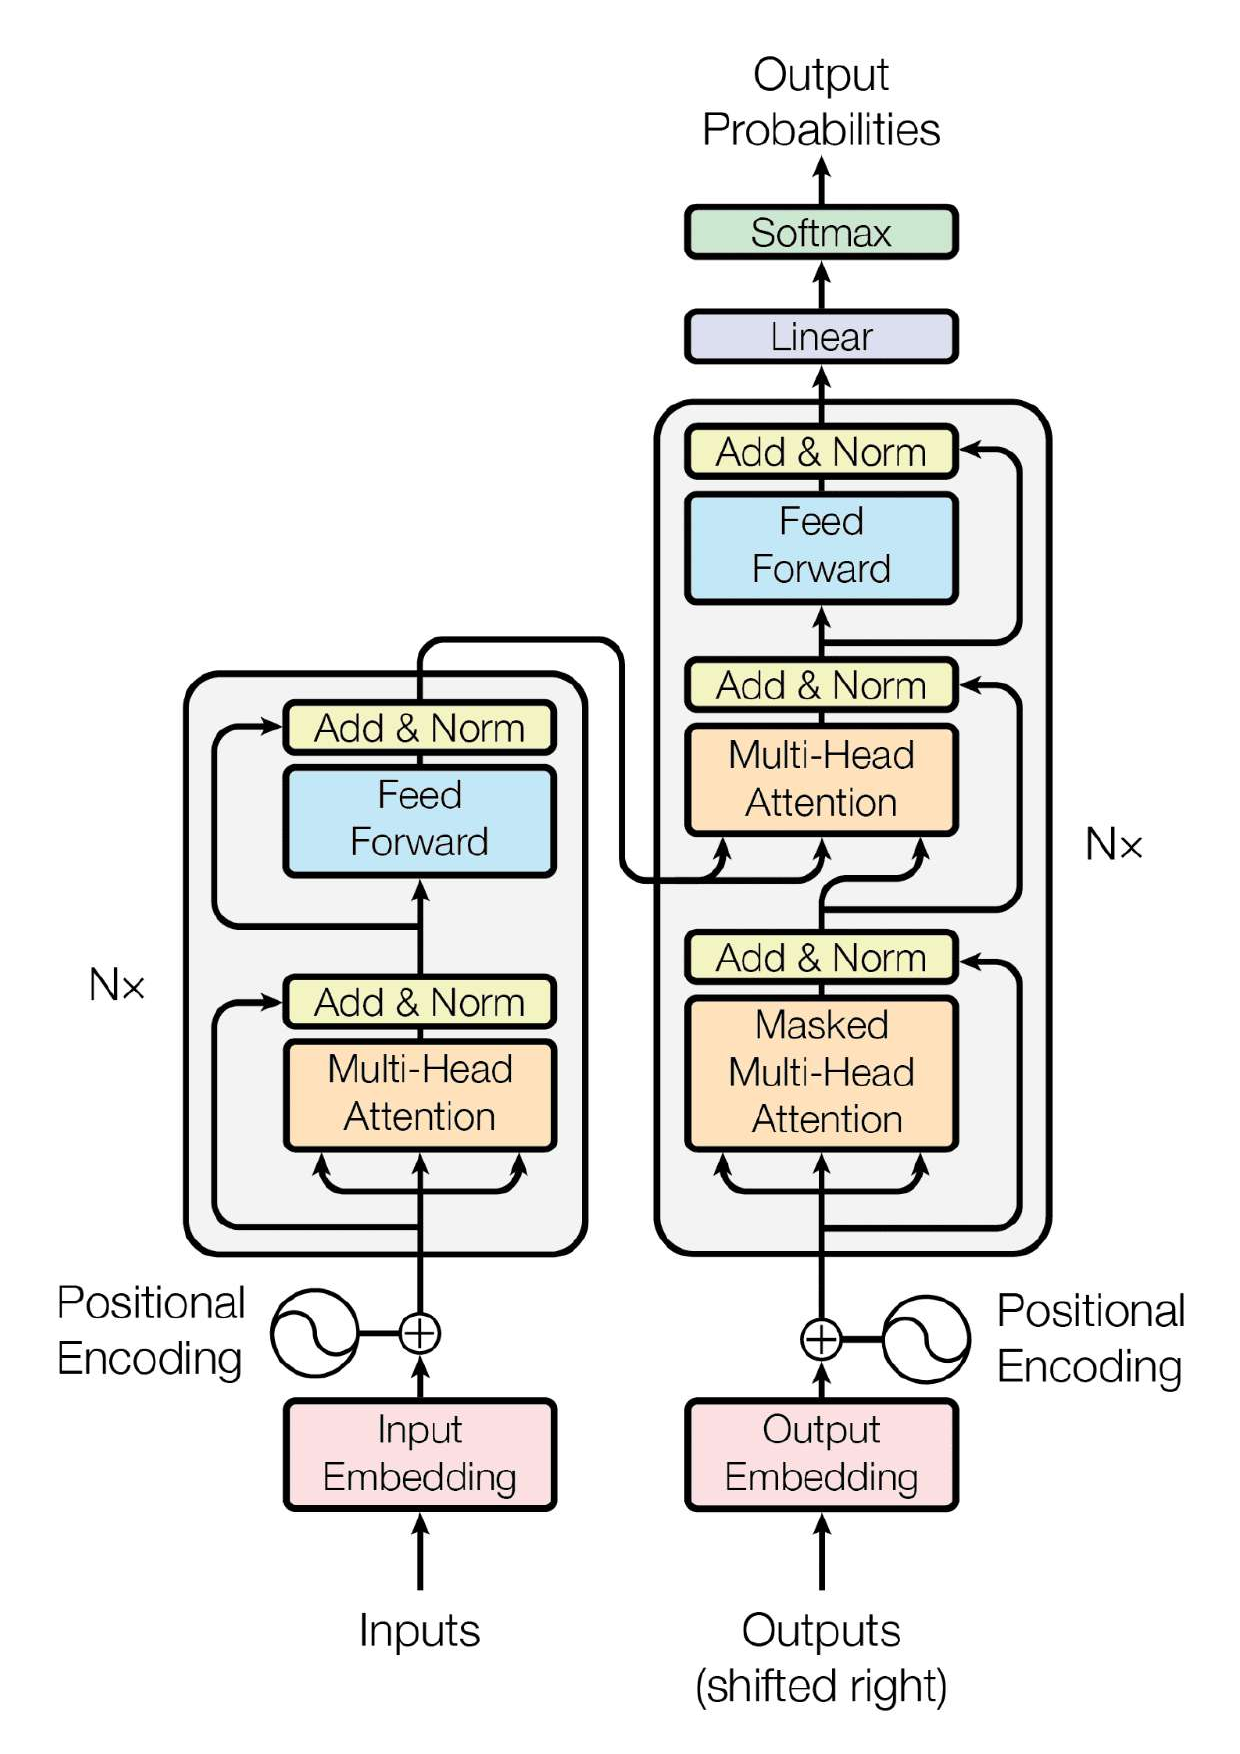
\includegraphics[width=10cm]{introduccion/figuras/Transformer_architecture.pdf}
\caption{The  encoder-decoder structure of the Transformer architecture. Taken from “Attention Is All You Need"}
\label{Transformer_architecture}
\end{figure}

\section{Examples of Applications in Other Fields}

Transformers have found applications beyond their original scope in Natural Language Processing (NLP). They are now widely used in various domains:

\par{Natural Language Processing (NLP):} Models such as BERT \cite{devlin2019bert} and GPT-3 \cite{brown2020language} leverage the Transformer architecture for tasks including language modeling, translation, and text generation. BERT (Bidirectional Encoder Representations from Transformers) is designed to pre-train deep bidirectional representations by jointly conditioning on both left and right context in all layers, which makes it particularly powerful for understanding the nuances of language. GPT-3 (Generative Pre-trained Transformer 3), on the other hand, is a state-of-the-art autoregressive language model capable of generating human-like text based on a given prompt, demonstrating the effectiveness of Transformers in creating coherent and contextually relevant text.

\par{Computer Vision:} Vision Transformers (ViTs) \cite{dosovitskiy2021image} apply the Transformer architecture to image classification tasks, achieving state-of-the-art performance by treating image patches as sequences of tokens. ViTs divide an image into a sequence of fixed-size patches, linearly embed each patch, add position embeddings, and then feed the resulting sequence of embeddings to a standard Transformer encoder. This approach allows ViTs to capture the global context of an image more effectively than traditional convolutional neural networks (CNNs), leading to impressive results on image recognition benchmarks.

\par{Audio Processing:} In the field of audio processing, Transformers are used for tasks such as speech recognition, audio generation, and music transcription. By treating audio signals as sequences, similar to text, Transformers can model long-range dependencies and capture temporal patterns more effectively than conventional methods.

\par{Protein Structure Prediction:} Transformers have made significant strides in the field of bioinformatics, particularly in protein structure prediction. The AlphaFold model \cite{Jumper2021HighlyAP} by DeepMind utilizes a Transformer-based architecture to predict the 3D structure of proteins from their amino acid sequences. This breakthrough has the potential to revolutionize biological research and drug discovery by providing accurate models of protein structures.

\par{Reinforcement Learning:} In reinforcement learning, Transformers are employed to model the sequential nature of decision-making processes. By leveraging their ability to handle long-range dependencies and parallelize computations, Transformers enhance the performance of reinforcement learning algorithms in various applications, from game playing to robotic control.

\par{Time-Series Forecasting:} Another significant application of Transformers is in the field of time-series forecasting. By treating time-series data as sequential input, Transformers can effectively model temporal dependencies and capture patterns over long time horizons. This makes them particularly well-suited for predicting future values in various domains, such as finance, weather forecasting, and inventory management.
